\documentclass{article}
\usepackage[a4paper, left=15mm, top=20mm, right=15mm,bottom=20mm]{geometry}
\usepackage{amsmath, amssymb, amsfonts}
\usepackage{fancyhdr}
\usepackage{graphicx}
\graphicspath{ {./images/} }
\usepackage{float}
\usepackage{hyperref}
\usepackage{lscape}

\pagestyle{fancy}
\fancyhf{}
\lhead{CS2040}
\rhead{claudeonrs}
\rfoot{\thepage}
\usepackage{amsmath, amssymb, amsfonts, listings}
\usepackage{xcolor}
\usepackage{enumitem}
\setlist[itemize]{noitemsep, topsep=0pt}
\setlist[enumerate]{noitemsep, topsep=0pt}
\setlist[description]{noitemsep, topsep=0pt}


%New colors defined below
\definecolor{codegreen}{rgb}{0,0.6,0.4}
\definecolor{codegray}{rgb}{0.5,0.5,0.5}
\definecolor{codepurple}{rgb}{0.58,0,0.82}
\definecolor{backcolour}{rgb}{0.95,0.95,0.92}
\definecolor{commentgreen}{rgb}{0.4,0.8,0.6}
%Code listing style named "mystyle"
\lstdefinestyle{mystyle}{
  backgroundcolor=\color{backcolour},
  commentstyle=\color{red},
  keywordstyle=\color{blue},
  numberstyle=\tiny\color{codegray},
  stringstyle=\color{codegreen},
  basicstyle=\ttfamily,
  breakatwhitespace=false,
  breaklines=true,
  captionpos=b,
  keepspaces=true,
  numbers=left,
  numbersep=5pt,
  showspaces=false,
  showstringspaces=false,
  showtabs=false,
  tabsize=2
}

%"mystyle" code listing set
\lstset{style=mystyle}

\title{No Title}
\author{Claudeon R Susanto}
\date{}
\usepackage[T1]{fontenc}
\usepackage[utf8]{inputenc}
\usepackage[english]{babel}
\usepackage{lmodern}

\renewcommand{\familydefault}{\sfdefault}   % Supprime le serif (dyslexie)
\usepackage[font=sf, labelfont={sf}]{caption}
\usepackage{multicol}
\usepackage{makecell}
\renewcommand\theadalign{bc}
\renewcommand\theadfont{\bfseries}
\renewcommand\theadgape{\Gape[4pt]}
\renewcommand\cellgape{\Gape[4pt]}



% own commands
\newcommand{\eg}[0]{\textit{e.g. }}
\newcommand{\ie}[0]{\textit{i.e. }}
\newcommand{\impt}[0]{\textcolor{red}{\textbf{[IMPT] }}}


\renewcommand\thesubsection{\thesection.\arabic{subsection}}
\setlength{\columnseprule}{1pt}
\begin{document}
%\maketitle
\fontfamily{lmss}\selectfont
\begin{multicols}{2}
\section{Introduction}
\textbf{Some questions to ask before starting on a problem}
\begin{itemize}
	\item Extract out important keywords (what DS to use?)
	\item Edge cases? \eg if \texttt{size==0} or \texttt{size==1},
	\item Trivial cases? can just hardcode
\end{itemize}
\textbf{Code styling}
\begin{itemize}
	\item \href{https://nus-cs2030.github.io/1718-s2/style/index.html}{CS2030 Code Styling Guide}
	\item \href{https://google.github.io/styleguide/javaguide.html}{Google Java Styling Guide}
	\item \textbf{Modularity}: use method to print answers inside main method
	\begin{lstlisting}[language=java]
	\\ print answer
	ans = simulate(n,k,m);
	printAns();	\end{lstlisting}
    \item \textbf{No global variables}
\end{itemize}
\section{Java}

How to throw exception?
\begin{lstlisting}[language=Java]
public class MyException extends Exception {
	private int var;
	public MyException(int var) {
		this.var = var
	}
	public int getVar() {
		return this.var;
	}
}

public class Main {
	public static void main(String[] args) {
		try {
			...
			throw new MyException(errorVar);
		} catch (MyException e) {
			System.out.println(e.getVar());
		}
	}
}\end{lstlisting}




\section{Data Structures}
$$O(1) < O(\log{(n)}) < O(n^c) \text{ where } c<1 $$
$$O(n) <  O(\log{(n!)}) = O(n\log{(n)}) < O(n^2)$$
$$O(n^k)[\text{ where } k>2] < O(k^n) [\text{ where } k\geq1] < O(n!) $$
\textbf{How to implement Data Structures?}
\begin{itemize}
	\item Composition: use well-known DS as an attribute of the implemented DS
	\item Inheritance: extends well-known DS
\end{itemize}
\subsection{Linked List}
\begin{itemize}
	\item Motivation: implementation of list using array needs to occupy contiguous memory space (can result in memory error)
	\item Variants of linked list:
	\begin{itemize}
		\item Tailed (need to maintain \texttt{head} and \texttt{tail})
		\item Circular
		\item Doubly linked (\texttt{prev} and \texttt{next} attributes for \texttt{ListNode})
	\end{itemize}
	\item How to find cycle?\\
	Answer: use fast and slow pointers
	\begin{lstlisting}[language=java]
		slow = slow.next;
		fast = fast.next.next;\end{lstlisting}
	\item \impt Drawing pictures is very important to visualize the program!
	\item Sometimes maintaining two pointers is good (especially for deletion)
	\begin{lstlisting}[language=Java]
Node head = new Node();
Node prev = head;
\end{lstlisting}
\end{itemize}

\textbf{Java API}: \texttt{ArrayList} or \texttt{LinkedList}
\begin{lstlisting}[language=Java]
	\\ constructor
	ArrayList<Integer> list = new ArrayList<Integer>();
\end{lstlisting}

\subsection{Stack}
\begin{lstlisting}[language=Java]
	// to construct an array of generics
	E[] arr = (E[]) new Object[size];
	/*
	// does not work
	E[] arr = new E[size]
	*/
\end{lstlisting}
\textbf{Uses}:
\begin{itemize}
	\item \impt Converting infix to postfix expression (Lecture 4 Slide 28)
	\item \impt Evaluating postfix expression
\end{itemize}

\subsection{Queue}

\textbf{Uses}:
\begin{itemize}
	\item \impt Breadth-first traversal of trees
	\item Sliding Window (especially important for contiguous blocks of stuff)
\end{itemize}
\textbf{Implementations}:
\begin{itemize}
	\item ArrayDeque: can remove from back and front
	\begin{itemize}
		\item However Java API does not allow random access
		\item Hence, need to implement our own (Lab 3C)
	\end{itemize}
\end{itemize}
\section{Recursion}
\impt \textbf{Recipe for recursion} (3 fingers)
\begin{enumerate}
	\item \underline{General recursive case}: identify simpler instances of the same problem
	\item \underline{Base case}: cases that we can solve without recursion
	\item Be sure that we are able to \underline{reach the simplest} instance so that we won't end up in infinite loop
\end{enumerate}
\textbf{Uses}
\begin{itemize}
	\item Insert item into sorted LinkedList
	\item Tower of Hanoi
	\item \impt Combination ($n$ choose $k$)
	\item Binary search
	\item Finding $k$-th smalles element (use pivot element \texttt{p})\\
	move elements \texttt{< p} to the left of \texttt{p}\\
	move elements \texttt{> p} to the right of \texttt{p}
	\item Printing all permutations of a String
\end{itemize}
\textbf{Overloading}: same function name but with different parameters (useful in Java)\\
\textbf{Backtracking}
\begin{itemize}
	\item Solving problems recursively by trying to build a solution incrementally, one piece at a time, removing those solutions that fail to satisfy the constraints of the problem at any point in time
	\item \eg Queens Lab 4B: board is fixed\\
	queens can be added or removed!
	\begin{lstlisting}[language=Java]
Pair pos = new Paid(i,j);
if (isValidBoard(pos, currentQueens)) {
	currentQueens.add(pos);
	solveQueens(n, queensLeft-1, currentQueens);
	currentQueens.remove(pos);
}
\end{lstlisting}
\end{itemize}
\section{Sorting}
Some definitions
\begin{itemize}
	\item \textbf{Sort key}: use particular value of an object to do comparison and sort
	\item \textbf{In-place}: requires only a constant amount of extra space during the sorting process
	\item \textbf{Stable}: relative order of elements with the same key value is preserved by the algorithm
\end{itemize}
\textbf{Some ideas used in sorting}:
\begin{itemize}
	\item Internal vs external sort
	\item Iterative vs recursive
	\item \underline{Comparison vs non-comparison based}\\
	\eg radix sort
	\item \underline{Divide and conquer}
\end{itemize}
\textbf{Applications}
\begin{itemize}
	\item Uniqueness testing
	\item Deleting duplicates
	\item Frequency counting
	\item Efficient searching
\end{itemize}
\begin{table}[H]
	\centering{
	\begin{tabular}{c|c|c}
		&
		Iterative &
		Recursive \\ \hline
		Comparison &
		\begin{tabular}[c]{@{}c@{}}Bubble,\\ Selection,\\ Insertion\end{tabular} &
		\begin{tabular}[c]{@{}c@{}}Quick,\\ Merge\end{tabular} \\ \hline
		\begin{tabular}[c]{@{}c@{}}Non-\\ comparison\end{tabular} &
		&
		Radix
	\end{tabular}
}
\end{table}
\subsection{Algorithms}
\subsubsection{Selection Sort}
Time complexity: $O(n^2)$\\
Limitation: Not stable
\subsubsection{Bubble Sort}
Time complexity: $O(n^2)$
\begin{itemize}
	\item Using flag: $O(n)$ \texttt{isSorted}, is the input already sorted?
\end{itemize}
\subsubsection{Insertion Sort}
Time complexity:
\begin{itemize}
	\item Best case: input already sorted ($O(n)$)
	\item Worst case: input reversely sorted ($O(n^2)$)
\end{itemize}
\subsubsection{Merge Sort}
Time complexity:
\begin{itemize}
	\item \texttt{merge(arr, left, mid, right)} is $O(right-left+1)$
	\item \texttt{merge} is called $\log{n}$ times
	\item Hence $O(n\log{n})$
\end{itemize}
Limitations:
\begin{itemize}
	\item Need temporary array to store values during the \texttt{merge} process (not in-place)
\end{itemize}
\subsubsection{Quick Sort}
Time complexity:
\begin{itemize}
	\item \texttt{partition()}
	\item \texttt{quicksort(a, i, p)}
	\item Worst case is when it is already sorted, so the first group (elements < p) is empty: $O(n^2)$
	\item Best case: occurs when array is divided into 2 equal halves
	\begin{itemize}
		\item Depth is $\log{n}$
		\item Each level takes $n$ comparisons (including swaps)
		\item Hence $O(n\log{n})$ which is also the average case
	\end{itemize}
\end{itemize}
Limitation: Not stable
\subsubsection{Radix Sort}
Treat each data as a character string: no comparison needed\\
\textbf{Trick}: sort by unit digit $\rightarrow$ tenth digit $\rightarrow$ hundredth and so on...\\
Time complexity:
\begin{itemize}
	\item Initialize 10 groups (queues) to group the elements
	\item Complexity is $O(dn)$ where $d$ is the maximum number of digits of the $n$ numeric strings in the array
\end{itemize}
Limitation: Not in-place

\subsubsection{Bucket Sort}
\textbf{How it works}:
\begin{itemize}
	\item There are $b$ buckets, and each element \texttt{arr} is inserted into bucket according to a function \eg \texttt{(int) arr[j]*10}
	\item Similar to radix sort but $b$ can be any number (base?)\\
	\eg Tut 5 Q 3(b) where $N \leq \texttt{arr[i]} \leq 3N$,  we can have $3N$ buckets $1,2,3, \dots, 3N$ so that each bucket contains only 1 element
	\item So only 1 pass is needed a.k.a. $O(3N)$ time
	\item Possible problem: takes up alot of space?
\end{itemize}
\begin{table}[H]
	\centering{
		\resizebox{\columnwidth}{!}{
			\begin{tabular}{c|c|c|c|c}
				& Worst Case     & Best Case      & In-place? & Stable? \\ \hline
				Selection                                               & $O(n^2)$       & $O(n^2)$       &           & No      \\ \hline
				Insertion                                               & $O(n^2)$       & $O(n)$         &           &         \\ \hline
				Bubble                                                  & $O(n^2)$       & $O(n^2)$       &           &         \\ \hline
				\begin{tabular}[c]{@{}c@{}}Bubble\\ (Flag)\end{tabular} & $O(n^2)$       & $O(n)$         &           &         \\ \hline
				Merge                                                   & $O(n \log{n})$ & $O(n \log{n})$ & No        &         \\ \hline
				Radix                                                   & $O(dn)$        & $O(dn)$        & No        &         \\ \hline
				Quick                                                   & $O(n^2)$       & $O(n \log{n})$ &           & No
			\end{tabular}
	}}
\end{table}

\subsection{Java Sorting}
For list/arrays:
\begin{itemize}
	\item To convert arrays to list use \texttt{Arrays.asList}
	\item \texttt{Arrays.sort} or \texttt{Collections.sort}
\end{itemize}
For others: use \texttt{Collections.sort(list, compObj)}
\begin{lstlisting}[language=Java]
import java.util.Comparator;
class ObjComparator implements Comparator<Obj> {
	public int compare(Obj o1, Obj o2) {
		// if positive, o1 > o2
		// if negative, o1 < o2
		// if zero,     o1 = o2
	}
    public boolean equals(Object obj) {
    	// check to see if we have the same comparator object
    	return this = obj;
    }
}\end{lstlisting}


\section{Hashing}
Map ADT: <key, value> pairs mapping with 3 basic operations
\begin{itemize}
	\item \textbf{Retrieval}: retrieve value using the given key
	\item \textbf{Insertion}: insert/replace a value using the given key
	\item \textbf{Deletion}: delete the <key, value> pair using the given key
\end{itemize}
\textbf{Hash Table}: data structure that uses a \textbf{hash function} to efficiently map keys to values, for efficient search and retrieval\\
Types of Tables:
\begin{itemize}
	\item Direct Addressing Table
	\begin{itemize}
		\item Restrictions:
		\begin{itemize}
			\item Keys must be \underline{non-negative integer values}
			\item Range of keys must be \underline{small}
			\item Keys must be \underline{dense}
		\end{itemize}
	\end{itemize}
    \item Hash Tables
    \begin{itemize}
    	\item Map large integers to smaller integers (mod?)
    	\item Map non-integers to integers
    	\item \textbf{Collision}: hash function does not guarantee two different keys go to two different slots\\
    	two different keys have the same \textbf{hash value}
    	\item \underline{Criteria of good hash functions}
    	\begin{itemize}
    		\item Fast to compute
    		\item Scatter keys evenly
    		\item Less collisions
    		\item Need less slots
    	\end{itemize}
        \item Perfect hash functions: \textit{one-to-one} mapping between keys and hash values \ie no collision occurs
        \item Minimal perfect hash functions: table size is the same as the number of keywords supplied
        \item \textbf{Uniform Hash functions}: distributes keys evenly in the hash table (e.g. mod, floor function)
        $$hash(k) = \left\lfloor \frac{km}{X}\right\rfloor \text{ where } k=0,1,2,\dots,X-1$$
        \begin{itemize}
        	\item Division method: map into a table with $m$ slots
        	$$hash(k) = k \text{ mod }m$$
        	\item Multiplication method:
        	\begin{enumerate}
        		\item Multiply by a constant real number $A$ between 0 and 1\\
        		\textit{*Knuth recommends} $A = 1/\phi=0.618033$ \textit{to minimize collisions}
        		\item Extract the fractional part
        		\item Multiply by $m$, the hash table size
        	\end{enumerate}
        $$hash(k) = \lfloor m (kA- \lfloor kA \rfloor ) \rfloor$$
        \end{itemize}
        \item How to choose $m$?\\
        * Pick a prime number close to a power of two\\
        * power of 10 or 2 are no good cos it's the same as extracting the last few digits of decimal/binary representation
        \item \textbf{Hashing of Strings}
        \begin{itemize}
        	\item Summing all the characters is no good: because strings with same letters but different orders will collide
        	\item How to solve: take into account order of characters!
        	\begin{lstlisting}[language=Java]
hash(s):
  sum=0
  for each character c in s:
    sum = sum*31+s
  return sum%m\end{lstlisting}
        \end{itemize}
        \end{itemize}
\end{itemize}
\subsection{Collision Resolution}
$$\alpha(\text{load factor}) = \frac{n (\text{total number of keys})}{m (\text{number of slots})}$$
$\alpha$ measures how full the hash table is\vspace{0.5em}\\
\textbf{Criteria of good collision resolution method}
\begin{itemize}
	\item Minimize clustering
	\item Always find an empty slot if it exists
	\item Give different probe sequences when 2 initial probes are the same (secondary hash function)
	\item Fast
\end{itemize}
\subsubsection{Separate Chaining}
\begin{itemize}
	\item Use LinkedList to store keys with the same slot location
	\item Ideally can sort the LinkedList based on key to aid in searching
\end{itemize}
\textbf{Some problems}:
\begin{itemize}
	\item find(key) and delete(key) takes $O(n)$ time
	\item $\alpha$ is the average length of the LinkedList and will increase when $n$ increases
	\begin{itemize}
		\item Hence it is good to keep $\alpha$ bounded $\Rightarrow$ reconstruct the whole table when $\alpha$ exceeds a bound
	\end{itemize}
	\item Not cache friendly
\end{itemize}
\subsubsection{Linear Probing}
Probe sequence:
\begin{lstlisting}
hash(key)
hash(key+1)%m
hash(key+2)%m ...
\end{lstlisting}
\begin{itemize}
	\item \textbf{Insert:}\\
	When we get a collision, we scan linearly for the next available slot and put the key there
	\item \textbf{Find:}\\
	Probe sequence increases linearly from hash(k) until current key is equal to the key we want to find
	\item \textbf{Delete}
	\begin{itemize}
		\item \impt Cannot simply remove a value because find() only works when contiguous cells are occupied
		\item So how? Use lazy deletion (three different states of a slot)
		\begin{itemize}
			\item Occupied
			\item Occupied but mark as deleted
			\item Empty
		\end{itemize}
	\end{itemize}
\end{itemize}
\textbf{Some problems:}
\begin{itemize}
	\item \textbf{Primary clustering}: Can create many consecutive slots, increasing running time of find/insert/delete $O(n)$
\end{itemize}
Modified linear probing: (\texttt{d} and \texttt{m} are co-primes) \underline{to avoid primary clustering}
\begin{lstlisting}
	hash(key)
	hash(key+1*d)%m
	hash(key+2*d)%m ...
\end{lstlisting}

\subsubsection{Quadratic Probing}
\begin{lstlisting}
	hash(key)
	hash(key+1^2)%m
	hash(key+2^2)%m ...
\end{lstlisting}
\textbf{Theorem of Quadratic Probing}
\begin{quote}
If $\alpha < 0.5$(half-full) and $m$ is prime, the we can always find an empty slot
\end{quote}
\textbf{Some problems}
\begin{itemize}
	\item When table is more than half-full, there can be endless looping!
	\begin{itemize}
		\item To avoid table half-full, we can \textbf{resize} the table
		\item Usually new $m = 2\times m$
		\item But also need to re-hash all existing keys (expensive operation)
	\end{itemize}
	\item \textbf{Secondary clustering}: if two keys have the same initial position, their probe sequences are the same, but not as bad as linear probing
\end{itemize}

\subsubsection{Double Hashing}
Use a secondary hash function
\begin{lstlisting}
	hash(key)
	hash(key+1*hash2(key))%m
	hash(key+2*hash2(key))%m ...
\end{lstlisting}
Note that the secondary hash function must not evaluate to 0 (otherwise it's the same as separate chaining if not worse because of infinite loop)
$$\text{hash}_2(\text{key}) = p - (\text{key} \text{ mod } p)$$

\section{Trees}
\textbf{Some terminologies}: ancestor, descendant, parent, sibling, child, root, leaf node
\begin{itemize}
	\item Internal node: has one or more children, but root node is not an internal node
	\item Level of a node: level of root is 0, depends on how far it is from the root
	\item Height: maximum level of the nodes
	\item Size: number of nodes
	\item \textbf{Binary tree}: each node has at most 2 ordered children
	\item \textbf{Full binary tree}: all nodes at level < $h$ have two children, where $h$ is the height of the tree
	\item \textbf{Complete binary tree}: full down to level $h-1$, with level $h$ filled in \underline{from left to right}
\end{itemize}
\textbf{Implementations}
\begin{itemize}
	\item Reference based
	\item Array based
	\begin{lstlisting}[language=java]
class BinaryTree {
	int root;
	int free; // free space
	TreeNode tree[];
}
	\end{lstlisting}
\begin{itemize}
	\item \underline{What is free space?}\\
	the last element where the slot is free, if there are multiple free slots, all the slots before the last will link towards the last one $\Rightarrow$ last one is the pointer of the free
	\item \underline{Representing complete tree} using an array: use heap?
	$$i_{left} = i*2+1, i_{parent} = i//2$$
\end{itemize}
\end{itemize}

\subsection{Traversals}
\subsubsection{Post-order traversal}
Traverse the root after traversing the left and right subtrees
\begin{lstlisting}[language=java]
postorder(T) {
	if T is not empty then {
		postorder(T.left)
		postorder(T.right)
		print(T.item)
}}
\end{lstlisting}
\subsubsection{Pre-order traversal}
Traverse the root before traversing the left and right subtrees
\begin{lstlisting}[language=java]
preorder(T) {
	if T is not empty then {
		print(T.item)
		postorder(T.left)
		postorder(T.right)
}}
\end{lstlisting}
\subsubsection{In-order traversal}
Traverse the root in between traversing the left and right subtrees (\textbf{Do a sweep from left to right})
\begin{lstlisting}[language=java]
inorder(T) {
	if T is not empty then {
		postorder(T.left)
		print(T.item)
		postorder(T.right)
}}
\end{lstlisting}
\subsubsection{Level-order traversal}
Traverse the tree level by level and from left to right (Queue is important)
\begin{lstlisting}[language=java]
levelorder(T) {
	if T is empty return
	Q = new Queue
	Q.enqueue(T)

	while Q is not empty {
		curr = Q.dequeue()
		print curr.item
		if curr.left is not empty {
			Q.enqueue(curr.left)
		} if curr.right is not empty {
		    Q.enqueue(curr.right)
        }
}}
\end{lstlisting}
\subsubsection{Evaluation of Expression Tree}
Note that post-order, in-order, and pre-order of expression tree will produce postfix, infix, and prefix expressions
\impt Recursive procedure!

\subsection{Binary Search Trees (BST)}
\textbf{Some interesting stuff}
\begin{itemize}
	\item We can construct an AVL Tree/BST from a sorted array in $O(N)$ time where $N$ is the size of the array
\end{itemize}
\textbf{Visualgo Hacks}:
\begin{itemize}
	\item Possible number of structurally different BSTs with $n$ distinct elements
	$$f(n) = \sum_{i=0}^{n-1}f(i)\times f(n-1-i)$$
	where $f(0) = 1$ and $f(1)=1$
	\item Minimum number of vertices in an AVL Tree of a given height $h$
	$$f(h) = f(h-1) + f(h-2) + 1$$
	where $f(1) = 2$ and $f(2) = 4$
\end{itemize}
\textbf{Some operations}: Usually $O(h)$, but note that it's possible that $h=n$ if it is skewed (hence need AVL Tree)
\begin{itemize}
	\item Find min/max element
	\item Search for $x$
	\item Insertion
	\item Deletion (3 cases)
	\begin{itemize}
		\item node to be deleted T has no children
		\item T has only 1 child (left)
		\item node to be deleted T has two children $\Rightarrow$ replace with \textbf{successor (smallest element in the right subtree)}
	\end{itemize}
    \item Successor/Predecessor\\
    \impt note that if this was to be implemented, we need a \texttt{.parent} attribute as an addition to the \texttt{.child attribute}
    \item Inorder traversal $\Rightarrow$ each node will be traversed not more than 3 times! wow
\end{itemize}

\subsection{AVL Trees}
\textbf{Property}:
\begin{itemize}
	\item At any node, the difference in height between left and right subtree is at most 1 (invariant)
	$$|h_l -h_r| \leq 1$$
	\item A height balanced tree with $N$ vertices has height $h < 2 \times \log_2(N) \Rightarrow h = O(\log(N))$
	\item Minimal AVL Tree of height $h$: having the height $h$ and fewest possible number of nodes
\end{itemize}
\vspace{0.5em}
\textbf{Operations}
\begin{itemize}
	\item \texttt{rotateRight()}/\texttt{rotateLeft()}
	\begin{figure}[H]
		\centering
		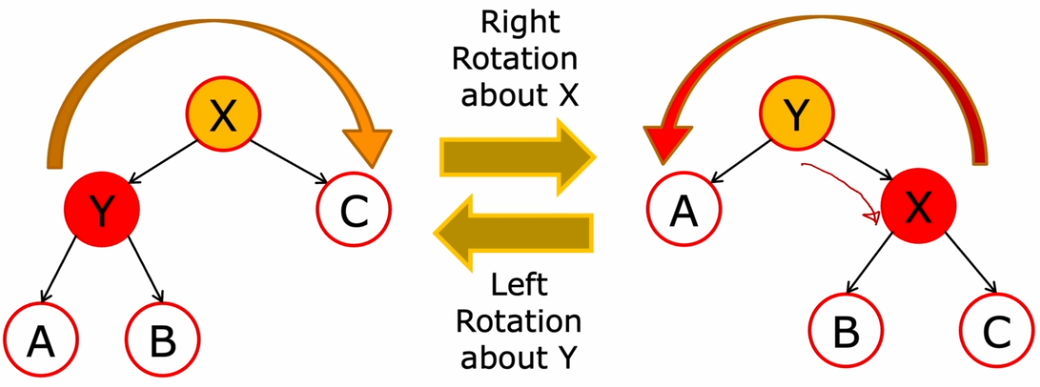
\includegraphics[width=\columnwidth]{image/avl_tree.png}
	\end{figure}
    \item \texttt{insert()}: do BST to find the appropriate node to insert to, then have two cases, and also need to pass through parents to see if they are height-balanced
    \begin{itemize}
    	\item insert outside: single rotation
    	\item insert inside: double rotation
    \end{itemize}
    \item Find $k$-th smallest item\\
    store \texttt{.size} attribute and do recursive stuff \impt \textbf{Quickselect} and partition on unsorted array\\
    \textbf{Running time}:
    \begin{itemize}
    	\item BST: $O(h)$
    	\item Unsorted array: Best case is $O(N)$, Worst case is $O(N^2)$
    \end{itemize}
\end{itemize}
\subsection{TreeMap Java API}
\begin{itemize}
	\item \texttt{higherkey()}, \texttt{floorkey()}: similar to predecessor and successor
	\item Has sorted key in tree structure
\end{itemize}

\section{Priority Queue}
\textbf{Property}
\begin{itemize}
	\item Insert item with a given key
	\item Remove the item with maximum key
\end{itemize}
\textbf{Implementations}
\begin{itemize}
	\item Unsorted list: insertion takes $O(1)$ but deletion takes $O(n)$ to remove the maximum key
	\item Sorted list: insertion takes $O(n)$ time but deletion takes $O(n)$ time
	\item Heap!
\end{itemize}
\subsection{Heap}
\textbf{VisuAlgo Hacks}
\begin{itemize}
	\item Maximum number of swaps between heap elements required to construct a max heap of $n$ elements using the $O(n)$ \texttt{BuildHeap(arrr)}: happens when the array is sorted in ascending order
	\item Maximum number of comparison between heap elements required to construct a max heap of $n$ elements using the $O(n)$ \texttt{BuildHeap(arrr)}
\end{itemize}
\textbf{Properties}:
\begin{itemize}
	\item A \textbf{complete binary tree}
	\begin{itemize}
		\item Either is empty,
		\item, or satisfies the \textbf{heap property}: for every node $v$, the search key in $v$ is greater or equal to those in the children of $v$
	\end{itemize}
    \item Usually we talk about max heap
    \item \impt Half of the items are leaves!
    \item Some access stuff
    \begin{lstlisting}[language=Java]
left(i)   = 2*i + 1
right(i)  = 2*i + 2
parent(i) = floor((i-1)/2)\end{lstlisting}
\end{itemize}
\textbf{Operations}
\begin{itemize}
	\item \texttt{heapRebuild(i)}: swap down from index $i$ until it reaches a leaf and satisfies the heap property
	\item \texttt{heapify()}: build a heap from an unsorted array (utilises \texttt{heapRebuild}) and is used for heapSort
	\begin{itemize}
		\item \textbf{Running time = }$O(n)$
		\item Total number of nodes = $n = 2^{h+1} - 1$
		\item Total number of bubbling down = $n-h-1$ which is less than the total number of edges connecting the nodes
		\item Worst case is when the array is sorted in ascending order (assuming max heap)
		\begin{lstlisting}[language=Java]
heapify(arr) {
	for (int i=size/2; i>=0; i--) {
		heapRebuild(i);
}}
\end{lstlisting}
	\end{itemize}

	\item \texttt{heapSort}: partition the unsorted array into two parts, the heap and sorted portion; remove the max value from heap and put it into the sorted portion so that eventually the array is in ascending order
	\begin{itemize}
		\item In-place
		\item Not stable (because of bubbling/swapping operations)
		\item Complexity = $O(n\log n)$
	\end{itemize}
\end{itemize}

\section{Union-Find Disjoint Sets (UFDS)}
\textbf{Definition}: collection of disjoin sets, ordering not important
\begin{itemize}
	\item Each set is modeled as a \underline{tree}
	\item A collection of disjoin sets forms a forest of trees
	\item Each set is represented by a representative item (root)
	\item \texttt{p[i]} records the parent of item \texttt{i}, if \texttt{p[i]==i}, then \texttt{i} is a root
\end{itemize}
\textbf{Operations}:
\begin{itemize}
	\item \texttt{unionSet(i,j)}: union two disjoin sets containing \texttt{i} and \texttt{j} respectively
	\begin{itemize}
		\item \textbf{Union-by-Rank} heuristic: make the resulting combined tree shorter by adding shorter tree to longer tree
		\item If height of trees are the same, we do not use this heuristic and just add normally
		\item Use another integer array \texttt{rank}
		\begin{itemize}
			\item \texttt{rank[i]} is the \texttt{upper bound} of the height of subtree rooted at \texttt{i}
		\end{itemize}
	\end{itemize}
    \begin{lstlisting}[language=Java]
unionSet(int i, int j) {
	if (!isSameSet(i,j)) {
		int x=findSet(i);
		int y=findSet(j);
		if (rank[x] > rank[y]) {
			p[y]=x; // add y to x
		} else {
		    p[x]=y; // add x to y
		    if (rank[x]==rank[y]) {
		    	rank[y]=rank[y]+1;
		    }
	    }
	}
}
\end{lstlisting}
	\item \texttt{findSet}: which set an item belongs to, trace recursively until \texttt{p[i]==i}
	\begin{itemize}
		\item Then we compress the nodes on the path to the root to make future find operations very fast $O(1)$
		\item Complexity is $O(\log{N})$, but with path compression can get to $O(1)$
	\end{itemize}
\begin{lstlisting}[language=Java]
findSet(int i) {
	if (p[i]==i) {
		return i;
	} else {
		p[i] = findSet(p[i]);
		return p[i];
	}
}
\end{lstlisting}
	\item \texttt{isSameSet(i,j)}: Check if two items belong to the same set
\end{itemize}
\subsection{Uses of UFDS}
\begin{itemize}
	\item \impt Detect Cycle in a graph!!!!
	\begin{itemize}
		\item Process edges one by one, union vertices if they have the same edge
		\item
	\end{itemize}
\end{itemize}

\section{Graphs}
\textbf{Properties}
\begin{itemize}
	\item Loops are possible; trees don't have loops
	\item Multiple paths are possible; Trees only have 1 path from A to B
\end{itemize}
\textbf{Types of graphs}
\begin{itemize}
	\item Weighted/Unweighted
	\item Directed/Undirected
	\item \textbf{Complete Graph}: Simple graph with $n$ vertices and $_nC_2$ edges
	\item Sparse/Dense: not so many edges vs many edges (arbitrary definition)
	\item Disconnected/Connected
\end{itemize}
\textbf{Some problems}
\begin{itemize}
	\item \underline{Shortest Path Problem}: What is the shortest way to travel between A and B?
	\item \underline{Traveling Salesman Problem}: How to minimize the cost of visiting $n$ cities such that we visit each city exactly once, and finishing at the city where we start from?
	\item \underline{Topological Sort}: Find a sequence of modules to take that satisfy the prerequisite requirements
	\item \underline{4-Colours Problem}
\end{itemize}
\subsection{Implementation}
\textbf{Some terminologies}
\begin{itemize}
	\item In/Out Degree of a vertex: for directed graph
	\item Cycle: only possible if there are \impt $geq n$ edges!!
	\item Path: number of \underline{edges} in a path
	\item Adjacent vertices: $adj(v)$ is a set of vertices adjacent to \texttt{v}
	\begin{itemize}
		\item For directed graphs
		$$\sum_v|adj(v)| = |E|$$
		\item For undirected graphs
		$$\sum_v|adj(v)| = 2|E|$$
	\end{itemize}
\end{itemize}
\textbf{Implementations}
\begin{itemize}
	\item Adjacency matrix: space complexity is $O(V^2)$
	\item Edge List: list all the edges (an Edge class) in a list space complexity is $O(E)$ where $E = O(V^2)$
	\item Adjacency List: stores all the neighbours of vertex A; space complexity is $O(V+E)$
	\item Vertex Map: similar to adjacency list but uses HashMap
\end{itemize}

\subsection{Traversal}
\subsubsection{BFS}
\begin{itemize}
	\item Use Queue for ordering
	\item How to differentiate visited vs univisited vertices?
	\begin{itemize}
		\item 1D array \texttt{visited} of size $V$, \texttt{visited[v]=0} initially, and \texttt{visited[v]=1} when \texttt{v} is visited
	\end{itemize}
    \item How to memorize the path?
    \begin{itemize}
    	\item 1D array \texttt{parent} of size $V$, where \texttt{p[v]} denotes the predecessor of \texttt{v}
    \end{itemize}
    \item The edges will form a spanning tree
    \item Running time is $O(E) + O(V) = O(V+E)$ if adjacency list is used (Main loop (secondary loop) + initialization inside first loop)
    $$O(\sum_{v}adj(curr)) = O(E)$$
    \item Running time is $O(V^2)$ if adjacency matrix is used
\end{itemize}
\textbf{Uses}:
\begin{itemize}
	\item \textbf{Building BFS Tree}
	\begin{lstlisting}[language=Java]
		Q = new Queue
		Q.enq(v)
		mark v as visited
		while Q is not empty {
			curr = Q.deq()
			print curr
			for each w in curr.adj { // an array of adjacent nodes
				if w is not visited {
					Q.enq(w)
					w.parent = curr
					mark w as visited
		}}}
\end{lstlisting}
    \item \textbf{Building BFS Tree}
    \begin{lstlisting}[language=Java]
    	Q = new Queue
    	Q.enq(v)
    	mark v as visited
    	v.level=0
    	while Q is not empty {
    		curr = Q.deq()
    		print curr
    		for each w in curr.adj { // an array of adjacent nodes
    			if w is not visited {
    				Q.enq(w)
    				w.level = curr.level+1
    				mark w as visited
    	}}}
\end{lstlisting}
\end{itemize}


\subsubsection{DFS}
\begin{itemize}
	\item Go to each path as far as we can go
	\item Use a stack
	\item Edges used in DFS traversal will form a DFS spanning tree
	\item $O(V+E)$
\end{itemize}
\begin{lstlisting}[language=Java]
S = new Stack
S.push(v)
print and mark v as visited
while S is not empty {
  curr = S.top() // top of stack
  if every vertex in adj(curr) is visited {
  	S.pop()
  } else {
    let w be an unvisited vertex in adj(curr)
    S.push(w)
    print and mark w as visited
}}
\end{lstlisting}

\subsubsection{Uses of BFS/DFS}
\begin{itemize}
	\item Searching for a vertex/node
	\item Reachability test: is v reachable from vertex u?
	\item Find shortest path between 2 vertices
	\item Identifying components (disconnected subgraphs)
	\begin{itemize}
		\item Run BFS on one node, and then label the visited vertices if they can be reached from the first node \eg 1,2,3,...
	\end{itemize}
    \item \impt Checking bipartite graph
    \item \impt Finding Spanning Tree
    \begin{itemize}
    	\item The tree is the MST if the edges are unweighted
    	\item If weighted, then maybe not
    \end{itemize}
    \item \textbf{Cycle Detection}: DFS!
    \begin{itemize}
    	\item Undirected: need to make sure that the path goes back to parent node
    	\begin{itemize}
    		\item \impt Running time is $O(V)$ if the graph is not necessarily connected; can just stop if there are more than $V-1$ edges traversed in that particular connected component
    		\item Possible false positive: two-nodes cycle, need to protect against this
    	\end{itemize}
        \item Directed: 3 states: unvisited, not completed, completed (Tut 9)
        \item \impt Alternatively can also use UFDS!
    \end{itemize}
    \item \textbf{Alternative DFS cycle detection in directed graph}
    \begin{itemize}
    	\item There is a cycle in a graph only if there is a back edge present in the graph
    	\item Check vertices currently in the recursion stack to detect back edge
    	\begin{itemize}
    		\item Basically check if we visit a vertex where it is on the path we are currently tracing
    	\end{itemize}
    \end{itemize}
	\item \textbf{Topological sort}: Module selection
	\begin{itemize}
		\item Should be a \textbf{Directed Acyclic Graph (DAG)}: a directed graph with no cycle since otherwise there will be a cycle where mods are prerequisites of each other
		\item Nice properties: if we go according to Topological Sort order, we ensure that the vertex will not be revisited again
		\item \textbf{Goal}: Order the vertices, such that if there is a path from $u$ to $v$, $u$ appears before $v$ in the output
		\item \textbf{Complexity}: $O(V+E)$
		\begin{lstlisting}[language=Java]
q = new Queue()
put all vertices with in-degree 0 into q
while q is not empty
  v = q.deq()
  print v
  remove v from G
  enqueue neighbours of v with in-degree 0\end{lstlisting}
	\end{itemize}
\end{itemize}

\subsection{Shortest Path}
\begin{itemize}
	\item \textbf{Path}: sequence of vertices $v_1, v_2, \dots, v_n$ where $(v_i, v_{i+1}) \in E$
	\item \textbf{Cost of a path}: sum of the cost of all edges in the path
	\item \textbf{distance(v)}: shortest distance from s to v
	\item \textbf{parent(v)}: previous node on the shortest path so far from s to v
	\item \textbf{weight(u, v)}: the weight of the edge from u to v
	\item BFS does not work because must track of the smallest distance so far
	\begin{itemize}
		\item Need to be able to backtrack and undo path if better solution is found
	\end{itemize}
\end{itemize}
\impt \textbf{Some other uses for SSSP}:
\begin{itemize}
	\item Can use Djikstra to compute minimax path (Lab 11A),
	\begin{itemize}
		\item Initialize \texttt{maxcap = 0} for all vertices, except \texttt{maxcap[src] = INFINITY}
		\item Relax operation updates the \texttt{maxcap} for each vertex (\texttt{cap} is the weight of edge connecting \texttt{u} and \texttt{v})
		\begin{lstlisting}[language=Java]
// maintains the maximum value of all the edges connected to v
maxcap[v] = max(maxcap[v], min(maxcap[u], cap))
\end{lstlisting}
	\end{itemize}
\end{itemize}
\subsubsection{Dijkstra Algorithm}
\textbf{Some observations} \impt
\begin{itemize}
	\item Set an attribute \texttt{distance} in each node, which measures (preliminary) distance from source to the node.
	\begin{lstlisting}[language=Java]
d = distance(v) + cost(v,w);
if (distance(w) > d) {
	// set distance to be d
	distance(w) = d;
	parent(w)=v
}
\end{lstlisting}
    \item Let v be a node with the minimum distance \texttt{distance(v)} out of all the unvisited nodes, then no matter how many times we call \texttt{relax}, the distance is still unchanged
\end{itemize}
\begin{lstlisting}[language=Python]
color all vertices yellow (uncompleted)
for each vertex w:
	distance(w) = INFINITY
distance(s) = 0
while there are yellow vertices:
	v = yellow vertex with the min distance (distance(v))
	color v red
	for each neighbour w of v:
		relax(v,w)
\end{lstlisting}
\textbf{Time complexity}
\begin{itemize}
	\item Total time complexity is $O((V+E)\log{V})$
	\item Initialization takes $O(V)$ time
	\item Remember that $\sum_{v}adj(v) = 2|E|$ so there would be $O(E)$ relax operations in total, where hopefully \texttt{relax} is $O(\log{V})$
	\item \impt \texttt{decreaseKey} need to be efficient (preferably $O(\log{V})$) so that \texttt{relax} can run in $O(\log{V})$ time
	\begin{itemize}
		\item Need to keep another array to keep track of where a specified node with id \texttt{w} is in the heap
		\item Or alternatively can store this attribute in the Vertex class
		\item \impt since PQ is not updated automatically when an item's priority is updated, then we need to call \texttt{decreaseKey} to update every time we update
	\end{itemize}
\end{itemize}
\begin{lstlisting}[language=Java]
// initialization is O(V)
for each vertex w {
	distance(w) = INFINITY;
}
distance(s) = 0;
pq = new PriorityQueue(V);

// main loop is O((V+E) log V)
while pq is not empty { // O(V)
	v = pq.deleteMin(); // O(log V) heap
	// means is colored red already
	for each neighbour w of v {
		//relax(v,w) // O(adj(v) * log V) in total
		// because when distance is updated, heap is not updated, so need to update manually using heapify() or heapRebuild
		d = distance(v) + cost(v,w);
		if (distance(w) > d) {
			// set distance to be d
			pq.decreaseKey(w,d);
			parent(w)=v
		}
}}
\end{lstlisting}

\subsubsection{Modified Dijkstra's Algorithm}
Key idea (\textbf{Lazy Data Structure}):
\begin{itemize}
	\item No \texttt{decreaseKey} operation, simply add the relaxed node to the PriorityQueue (allow duplicate nodes in the PQ)
	\item Since the relaxed node has lower weight anyways
	\item If the node is extracted already, mark other nodes with same IDs as processed already
	\item Optimization: Once we have finalized $|V|$ nodes, we can stop already
	\item Running time: $O(V+E)\log{V}$
	\begin{itemize}
		\item Initialization is $O(V)$
		\item The number of edges is an upper bound on the queue size (we can relax each edge maximum once)
		\item Upper bound for the number of edges is $|E|= |V|^2$
		\item Each enqueue/dequeue operation is $O(\log{|E|}) = O(\log{|V|^2}) = O(\log{|V|})$ where $|E|$ is the max queue size
		\item Same complexity as original Dijkstra, but probably a constant factor difference
	\end{itemize}
\end{itemize}
\begin{lstlisting}[language=Java]
for each vertex w {
	D[w] = INFINITY; // distance array
}
D[s] = 0;
pq = new PriorityQueue();
pq.push(s,0); // enqueue source
count = |V|; // optimization

while (pq.isEmpty() && count > 0) {
	(d,u) = pq.deleteMin();
	if (d == D[u]) {
		count--;
		foreach neighbour w of u {
			if (D[w] > D[u] + cost(u,w)) {
				D[w] = D[u] + cost(u,w); // relax
				pq.push((D[w],w)); // push to pq
				parent(w) = u;
			}
		}
	}
}
\end{lstlisting}

\subsubsection{Bellman-Ford Algorithm}
\begin{itemize}
	\item Dijkstra's Algorithm does not allow negative weights as the vertex with minimum distance is already considered as finalized
	\begin{itemize}
		\item Can deal with negative weight cycles (detection)
		\item Can detect negative weight cycles
		\item Is quite simple (no special data structure needed)
		\item but has higher runtime complexity than Dijkstra
	\end{itemize}
	\item Negative cycle is a special case (a cycle that sums up to negative number) since we can traverse the cycle an infinite number of times to get a $- \infty$ cost of path
	\item Complexity is $O(VE)$ which can reach up to $O(V^3)$ if $E \sim V^2$
	\item Use an edge list (don't need to be sorted)
	\begin{lstlisting}[language=java]
class Edge {
	int src, dest, weight;
	Edge() {
		src = dest = weight = 0;
	}
}

// edge list
int V, E;
Edge[] Edge;
\end{lstlisting}
    \item Initialization $O(V)$: set the distance of every node to infinite except src
    \begin{lstlisting}[language=Java]
int[] dist = new int[V];
for (int i==0; i<V; ++i) {
  dist[i] = Integer.MAX_VALUE;
}
dist[src] = 0;
\end{lstlisting}
    \item Do the following $|V-1|$ times: relax each edge in every round, each round is $O(E)$ which means in total we have $O(VE)$
    \begin{lstlisting}[language=Java]
// relax
if (dist[v] > dist[u] + weight of edge uv) {
	// update dist[v]
	dist[v] = dist[u] + weight of edge uv;
}
\end{lstlisting}
\item \impt Last round ($V^{th}$ round) is used to check \textbf{negative weight cycle}
\begin{itemize}
	\item If there is anymore changing edgeweight, then it has negative cycle and thus not valid
\end{itemize}
\end{itemize}
\subsection{Minimum Spanning Tree (MST)}
\textbf{MST Problem}: given connected graph $G$ with positive edge weights, find a minimum weight set of edges that connects all of the vertices
\begin{itemize}
	\item Note that a tree of a graph $G$ has $|V|$ number of edges
	\item Minimize total costs to connect every single vertex
\end{itemize}
\impt Uses of MST Algorithms
\begin{itemize}
	\item Find the path which contains the max minimum edge to maximize capacity (Lab 11A)
	\item Find the most difficult cell along the easiest path (Tut 10.1)
\end{itemize}
\subsubsection{Kruskal's Algorithm}
\textbf{Greedy algorithm!}: it works because the tree will confirm have $|V|-1$ edges
\begin{enumerate}
	\item Sort all edges in non-decreasing order of their weight (from smallest to largest)
	\begin{itemize}
		\item Edge List representation is useful
	\end{itemize}
    \item Pick the smallest edge
    \item Check if it forms a cycle with the spanning tree formed so far. If cycle is not formed, include this edge, else, discard it
    \begin{itemize}
    	\item Cycle detection uses UFDS
    \end{itemize}
    \item Repeat step 2-3 until there are $(|V|-1)$ edges in the spanning tree
\end{enumerate}
\textbf{Complexity}
\begin{itemize}
	\item Sorting of Edges takes $O(E \log{E})$ time
	\item Iterating through all edges and apply union-find algorithm takes at most $O(\log{V})$ per edge, so $O(E\log{V})$
	\item Overall complexity is $O(E\log{E} + E\log{V}) = O(E\log{V})$
\end{itemize}

\subsubsection{Prim's Algorithm}
\textbf{Key Idea}"
\begin{enumerate}
	\item Start with an empty spanning tree
	\item Maintain two sets of vertices
	\begin{itemize}
		\item 1st set contains the vertices in the MST
		\item 2nd set contains vertices not yet included
	\end{itemize}
    \item At every step, consider all the edges that connect the two sets, and pick the minimum weight edge from these edges
    \begin{itemize}
    	\item Conceptually similar to Dijkstra as we finalize some edges
    	\item \textbf{Graph cut}: a group of edges that connects two sets of vertices in a graph
    	\item At this step we need to find the minimum weight edge from the cut and include this vertex into the MST
    \end{itemize}
    \item Move the other endpoint of the edge to the set containing the MST
\end{enumerate}
\textbf{Procedure/Algorithm}
\begin{enumerate}
	\item Initialize an array \texttt{parent} and \texttt{weight} that keeps track of the weight and parent
	\begin{itemize}
		\item The parent array is the output which is used to show the constructed MST
	\end{itemize}
	\item Create a set \texttt{mstSet} that keeps track of vertices already included in the MST
	\item Assign a key value to all vertices in the graph
	\begin{itemize}
		\item The first vertex has key value 0
		\item The rest have key value $\infty$
	\end{itemize}
    \item While \texttt{mstSet} does not include all vertices, do the following:
    \begin{enumerate}
    	\item Pick a vertex $u$ which is not in \texttt{mstSet} and has minimum key value
    	\item Include $u$ into \texttt{mstSet}
    	\item Update key values of all adjacent vertices of $u$
    	\begin{itemize}
    		\item For every adjacent vertex $v$, if weight of edge $u\leftrightarrow v$ is less than the previous key value of $v$, update the key value as weight$(u\leftrightarrow v)$
    	\end{itemize}
    \end{enumerate}
\end{enumerate}
\textbf{Complexity}
\begin{itemize}
	\item $O(V^2)$ if the input graph is represented using an adjacency list
	\item With binary heap, can be reduced to $O(E\log{V})$ (same as Kruskal's)
\end{itemize}

\section{Java Tricks}
\begin{itemize}
	\item OOP is important (CardGame)
	\begin{itemize}
		\item If it involves an array, OOP is useful, methods can just modify properties/attributes of the object class (\eg \texttt{reversed=true; increment=4})
		\begin{itemize}
			\item Especially true if only need to print statement at the end
		\end{itemize}
	\end{itemize}
	\item Invariance: property that stays constant???\\
	Lab 5C: Pancakes: Use number of inversions if it's even or not
	\item Use \texttt{StringBuilder} for return statements
	\begin{itemize}
		\item \href{https://docs.oracle.com/javase/7/docs/api/java/lang/StringBuilder.html}{Java StringBuilder API}
		\item \href{https://leetcode.com/problems/zigzag-conversion/solution/}{Zigzag conversion}
	\end{itemize}
    \item Tut 07 $\Rightarrow$ Contiguous cells can be represented by start and end only
    \item \impt \textbf{Iterator}
    \begin{lstlisting}[language=Java]
LinkedList<Integer> ll = new LinkedList<>();
Iterator<Integer> it = ll.iterator();
it.next();
// must call next first before removing;
it.remove();
it.next();
// must call next first
it.remove();
\end{lstlisting}
    \item \textbf{Mix and Match}:
    \begin{itemize}
    	\item Sometimes it's useful to combine two data structures rather than maintaining two separate DS
    	\begin{itemize}
    		\item \eg BST + Sorted List for easy successor and printOrder access
    		\item \eg Queue + Doubly Linked List + BST
    	\end{itemize}
    \end{itemize}

\end{itemize}

\end{multicols}






\end{document}